\documentclass[11pt,a4paper]{amsart}

\usepackage[margin=1in]{geometry}
\usepackage{graphicx}
\usepackage{amsmath}
\usepackage{amsfonts}
\usepackage{amsthm}
\usepackage{mathrsfs}
\usepackage{float}
\usepackage{subfig}
\usepackage{hyperref}
\usepackage{dsfont}

\makeatletter
\def\dual#1{\expandafter\dual@aux#1\@nil}
\def\dual@aux#1/#2\@nil{\begin{tabular}{@{}c@{}}#1\\#2\end{tabular}}
\makeatother


\newtheorem{thm}{Theorem}[section]
\newtheorem{ex}{Example}
\newtheorem{prb}{Problem}
\newtheorem{pf}{Proof}
\newtheorem{lem}[thm]{Lemma}
\newtheorem{prop}[thm]{Proposition}
\newtheorem{cor}[thm]{Corollary}
\newtheorem{conj}[thm]{Conjecture}
\newtheorem{defn}{Definition}[section]
\newtheorem{example}{Example}[section]

\newcommand{\PP}{\mathbb{P}}		%Used for probabilities.
\newcommand{\NN}{\mathbb{N}}		%Used to denote the natural numbers.
\newcommand{\RR}{\mathbb{R}}		%Used to denote the real numbers.
\newcommand{\statespace}{\mathscr{S}}	%Used to denote the state space.
\newcommand{\MM}{\mathscr{M}}		%Used to denote the space of measurable sets.
\newcommand{\CC}{\mathbb{C}}
\DeclareMathOperator{\Var}{\text{Var}}
\newcommand{\s}{\sigma}
\newcommand{\W}{\widetilde{W}}
\newcommand{\w}{\omega}
\newcommand{\EE}{\mathbb{E}}
\newcommand{\N}{\mathcal{N}}


\begin{document}
\title{Monte Carlo Methods: HW 4}
\author{Terrence Alsup}
\date{April 17th, 2019}
\maketitle

%\emph{Note: The MCMC methods are implemented in the Python file {\tt IsingSamplers.py}}.

%\vspace{0.5in}

%%%%%%%%%%%%%%%%%%%%%%%%%%%%%%%%%%%%%%

{\bf Exercise 60}\\
\\
\par The Python file {\tt XYmodel.py} contains a class called {\tt XYmodel}, which is a sample from the distribution
\[
\pi(\vec{\sigma}) = \frac{1}{Z} \exp\left(\beta \sum_{i \leftrightarrow j} \vec{\sigma}_i \cdot \vec{\sigma}_j \right),
\]
and contains methods to evaluate $\log \pi$ and $\nabla \log \pi$ for instance.  It also contains methods to compute the magnetization vector
\[
M(\sigma) = \sum_{i=0}^{L-1} \vec{\sigma}_i
\]
and the cosine of its angle $\frac{M_1(\sigma)}{\|M(\sigma)\|_2}$.  Since we have the constraint $\|\vec{\sigma}_i\|_2 = 1$ we do MCMC on the corresponding angles $\theta_i$.  In particular, we update the angles $X = (\theta_1,\ldots,\theta_L)$ based on
\[
X_h^{(k+1)} = X_h^{(k)} + h\nabla^T\log \pi(X_h^{(k)}) + \sqrt{h} \xi^{(k+1)}.
\]
Note that we have taken $S = I$ and $\xi \sim N(0, I)$.  The limit of the generator of this process is the overdamped Langevin operator.  This scheme is implemented in the Python file {\tt ex60\_alsup.py}.  Figures~\ref{fig:sample_b1} and \ref{fig:sample_b10} below show 2 different samples of the XY model when $\beta$ is relatively small and relatively large, respectively.  We see that for small $\beta$, meaning high temperatures, the vectors are much less clustered.  On the other hand, for large $\beta$, meaning low temperatures, we see that all of the vectors have clustered together.  If the particles were completely independent then the probability that $L=25$ particles all fall on the same half of the unit circle is
\[
\left( \frac{1}{2} \right)^{L-1} \approx 5.96 \times 10^{-8},
\]
suggesting that the MCMC is at least drawing samples from some distribution close to $\pi$.\\

\begin{figure}[H]
\centering
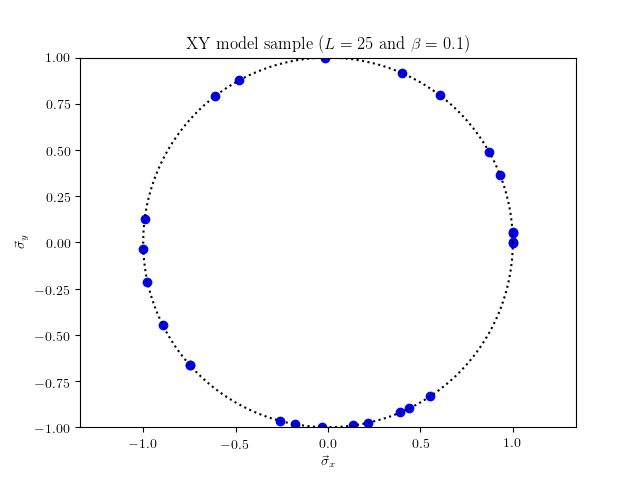
\includegraphics[width=5in]{sample_b1.png}
\caption{A random sample from the XY model with $L=25$ and $\beta = 0.1$.  We have done $N = 10^4$ un-metropolized MCMC steps with step-size $h = 10^{-2}$.}
\label{fig:sample_b1}
\end{figure}

\begin{figure}[H]
\centering
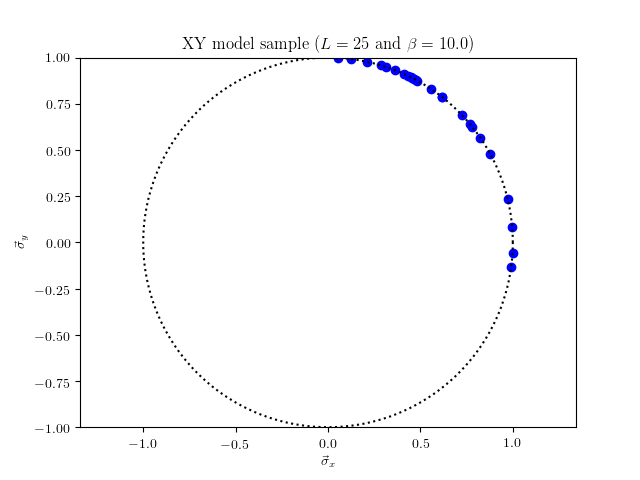
\includegraphics[width=5in]{sample_b10.png}
\caption{A random sample from the XY model with $L=25$ and $\beta = 10$.  We have done $N = 10^4$ un-metropolized MCMC steps with step-size $h = 10^{-2}$.}
\label{fig:sample_b10}
\end{figure}



\par We can compare the Metropolized and un-Metropolized schemes for different values of $h$ by looking at the integrated autocorrelation times (IAC) as in Table~\ref{table:IAC_OL}.  For smaller $h$ the IAC is much higher for both schemes and is more difficult to estimate.  The IAC for both the Metropolized and un-Metropolized schemes are about the same, although for Metropolized it is a little bit higher on average.  This seems reasonable since more rejections causes the chain to barely move.  We also see that for smaller $h$ the rejecction rate decreases so for $h\approx 0$ the two chains are more or less equivalent since we will never reject.  $h = 0.5$ seems to be a good trade-off in terms of minimizing IAC and maximizing acceptance rate.  We note that for each step of the algorithm we require 1 evaluation of $\nabla \log \pi$ for un-Metropolized and 2 evaluations for Metropolized.\\


\begin{table}[H]
\centering
\begin{tabular}{l | r r r}
$h$ & Un-Metropolized & Metropolized & Rejection Rate (\%) \\
\hline
$5 \times 10^{-2}$ & 69.9 & 64.6 & 2.51\\
$10^{-1}$ & 22.6 & 37.7 & 4.21 \\
$5\times 10^{-1}$ & 8.1 & 8.4 & 10.15 \\
$1$ & 4.6 & 5.8 & 14.59
\end{tabular}
\caption{Estimated IAC's for the Metropolized and un-Metropolized overdamped Langevin MCMC schemes.  Here $L=25$ and $\beta=0.1$.  For each $h$ we estimate the IAC by running chains of length $N = 10^3,10^4$, and $10^5$ to check for convergence.  For the Metropolized scheme we also give the rejection rate.}
\label{table:IAC_OL}
\end{table}

\par In addition to changing the step size $h$, we can also see how the number of particles $L$ affects these schemes.  Table~\ref{table:IAC_OL_L} below shows this dependence.  We see that increasing $L$ does not affect the IAC for the un-Metropolized scheme.  However, the un-Metropolized scheme is biased, and this bias gets worse as we increase the dimension $L$.  This is reflected in the results for the Metropolized scheme as well, which is unbiased.  For the Metropolozed scheme, we have to correct for the larger bias, which is also why the rejection rates are increasing.  Unless we want to use a much smaller time step $h$, it would probably be better to use the Metropolized scheme.

\begin{table}[H]
\centering
\begin{tabular}{l | r r r}
$L$ & Un-Metropolized & Metropolized & Rejection Rate (\%) \\
\hline
$25 $ & 8.1 & 8.4 & 10.15\\
$50$ & 9.2 & 13.5 & 16.20 \\
$100$ & 7.6 & 12.5 & 22.85 \\
$250$ & 7.5 & 17.0 & 37.85
\end{tabular}
\caption{Estimated IAC's for the Metropolized and un-Metropolized overdamped Langevin MCMC schemes.  Here $\beta=0.1$ and $h=0.5$.  For each $L$ we estimate the IAC by running chains of length $N = 10^3,10^4$, and $10^5$ to check for convergence.  For the Metropolized scheme we also give the rejection rate.}
\label{table:IAC_OL_L}
\end{table}


%%%%%%%%%%%%%%%%%%%%%%%%%%%%%%%%%%%%%%

{\bf Exercise 61}\\
\\
\par An alternative to using overdamped Langevin is to use Hybrid Monte Carlo with a velocity verlet integrator.  In our case, we set
\[
K(\tilde{x}) = \frac{1}{2}\|\tilde{x}\|^2 \quad \text{ and } \quad \hat{J} = I.
\]
For $n$ steps of velocity verlet, we require approximately $2n$ evaluations of $\nabla \log \pi$ since we can re-use one of the evaluations for the next step.  Thus, we cannot take $n$ to be too large.  For the implementation contained in the Python file {\tt ex61\_alsup.py} we take $n=5$.  Since we require $n$-times more evaluations than the overdamped Langevin sampler we can compare the methods by looking at the ratio of cost and effective sample size.  For a chain of length $N$, the effective sample size is roughly defined as
\[
N_{\text{eff}} = \frac{N}{\tau}
\]
where $\tau$ is the IAC time.  The total cost is just $2 \times n \times N$ and the approximate ratio of cost per effective sample is 
\[
\frac{\text{cost}}{N_{\text{eff}}} = \frac{2\times n \times N}{N/\tau} = 2\times n \times \tau
\]
Note that for larger $n$, the cost of the algorithm is dominated by the cost in the velocity verlet integrator and not in computing the acceptance probability.  Thus, the total cost for Metropolized and un-Metropolized is essentially the same. Table~\ref{table:IAC_HMC} shows how the Metropolized and un-Metropolized Hybrid Monte Carlo schemes compare to each other in terms of IAC time for different values of $h$.  We see that the IAC times are nearly $1$ for large step sizes.  Because $\beta = 0.1$ is small the samples in the chain decorrelate quickly.  Consider the extreme case when $\beta = 0$, then $\pi$ is just the uniform distribution and we can just draw i.i.d. samples.  Again as we would expect the rejection rate also increases as we increase the step size $h$.

\begin{table}[H]
\centering
\begin{tabular}{l | r r r}
$h$ & Un-Metropolized & Metropolized & Rejection Rate (\%)\\
\hline
$5\times 10^{-2} $ &  36 & 37.3 & 0.01 \\
$10^{-1}$               &  11.7  & 16.3 & 0.07 \\
$5\times 10^{-1} $ &  $\approx 1$ & 1.20 & 1.40 \\
$1$                           & $\approx 1$ & $\approx 1$ & 5.86
\end{tabular}
\caption{Estimated IAC's for the Metropolized and un-Metropolized Hybrid Monte Carlo MCMC schemes.  Here $\beta=0.1$ and $L=25$.  For each $h$ we estimate the IAC by running chains of length $N = 10^3,10^4$, and $10^5$ to check for convergence.  For the Metropolized scheme we also give the rejection rate.}
\label{table:IAC_HMC}
\end{table}



\par Table~\ref{table:cost_per_sample_HMC} below shows the cost to effective sample ratio for Hybrid Monte Carlo compared with the Metropolized overdamped Langevin scheme.  The Hybrid Monte Carlo only pays off if we take a relatively large step size $h$ otherwise it is cheaper just to use the overdamped Langevin.  However, we expect Hybrid Monte Carlo to be better suited for larger $\beta$ where the IAC is more difficult to estimate for the overdamped Langevin sampler.

\begin{table}[H]
\centering
\begin{tabular}{l | r r }
$h$ & \dual{Hybrid Monte Carlo/ \text{Approximate Cost/Sample}} & \dual{Overdamped Langevin/ \text{Approximate Cost/Sample}} \\
\hline
$5\times 10^{-2} $ & 373 & 129\\
$10^{-1}$ & 163 & 75 \\
$5\times 10^{-1}$ & 12 & 16 \\
$1$ & 9 & 11
\end{tabular}
\caption{Estimated cost per effective sample for the Metropolized Hybrid Monte Carlo and overdamped Langevin MCMC schemes.  Here $\beta=0.1$, $L=25$, $N=10^4$.  For the Hybrid Monte Carlo $n=5$, $\hat{J} = I$, and $K(x) = \|x\|^2/2$.}
\label{table:cost_per_sample_HMC}
\end{table}


%%%%%%%%%%%%%%%%%%%%%%%%%%%%%%%%%%%%%%

{\bf Exercise 62}\\
\\
\par The Python file {\tt ex62\_alsup.py} implements an underdamped Langevin sampler for the XY model.  We again take $\beta =0.1$ and $L=25$.  Table~\ref{table:IAC_UL} shows the dependence of the IAC time $\tau$ on the step size $h$ for the Metropolized and un-Metropolized schemes.  We see that these are slightly smaller than the overdamped Langevin sampler, but also slightly larger than the Hybrid Monte Carlo scheme.  Of course, we can perhaps get a better scheme by changing the friction coefficient $\gamma$.  The results are displayed in Table~\ref{table:IAC_friction} below.  We see that increasing the friction $\gamma$ results in a larger IAC time, but the addition of any friction also reduces the rejection rate.  


\begin{table}[H]
\centering
\begin{tabular}{l | r r r}
$h$ & Un-Metropolized & Metropolized & Rejection Rate (\%)\\
\hline
$5\times 10^{-2} $ &  56.2 & 56.0 & 0.01 \\
$10^{-1}$               &  35.6  & 29.3 & 0.02 \\
$5\times 10^{-1} $ &  6.7 & 9.4 & 1.53 \\
$1$                           & 3.1 & 4.5 & 7.51
\end{tabular}
\caption{Estimated IAC's for the Metropolized and un-Metropolized underdamped Langevin MCMC schemes.  Here $\beta=0.1$ and $L=25$.  We also set the friction coefficient $\gamma = 1$.  For each $h$ we estimate the IAC by running chains of length $N = 10^3,10^4$, and $10^5$ to check for convergence.  For the Metropolized scheme we also give the rejection rate.}
\label{table:IAC_UL}
\end{table}



\begin{table}[H]
\centering
\begin{tabular}{l | r r r}
$\gamma$ & Un-Metropolized & Metropolized & Rejection Rate (\%)\\
\hline
$10^{-1}$  & 22.0  & 29.1   & 0.02\\
$1$              & 25.5  & 33.9   & 0.04\\
$10$            & 55.4  & 60.2   & 0.11\\
$50$            &  100.3 & 166.6 & 0.06
\end{tabular}
\caption{Estimated IAC's for the Metropolized and un-Metropolized underdamped Langevin MCMC schemes.  Here $\beta=0.1$ and $L=25$.  We also set the step size $h = 0.1$.  For each $\gamma$ we estimate the IAC by running chains of length $N = 10^3,10^4$, and $10^5$ to check for convergence.  For the Metropolized scheme we also give the rejection rate.}
\label{table:IAC_friction}
\end{table}

\par In contrast to the verlet integrator in Hybrid Monte Carlo we do not need to $O(n)$ evaluations of $\nabla \log \pi$ at each step in the chain.  This means that it will be much cheaper to evaluate when $n$ is even moderate.  However, it is still slightly more expensive than the overdamped Langevin sampler.  If we re-use values between steps we require approximately $2$ evaluations of $\nabla \log \pi$ per step.  Thus, for the over and underdamped Langevin equations we compute the cost per effective sample as $2 \times \tau$.  Table~\ref{table:cost_per_sample} shows the cost per effective sample for the Metropolized versions of all of these schemes.

\begin{table}[H]
\centering
\begin{tabular}{l | r r r }
$h$ & \dual{Hybrid Monte Carlo/ \text{Approximate Cost/Sample}} & \dual{Overdamped Langevin/ \text{Approximate Cost/Sample}} &  \dual{Underdamped Langevin/\text{Cost/Sample}} \\
\hline
$5\times 10^{-2} $ & 373 & 129 & 112 \\
$10^{-1}$ & 163 & 75 & 68 \\
$5\times 10^{-1}$ & 12 & 16 & 19 \\
$1$ & 9 & 11 & 9
\end{tabular}
\caption{Estimated cost per effective sample for the Metropolized MCMC schemes.  Here $\beta=0.1$, $L=25$, $N=10^4$.  For the Hybrid Monte Carlo $n=5$, $\hat{J} = I$, and $K(x) = \|x\|^2/2$.  For the underdamped Langevin we have set $\gamma = 1$.}
\label{table:cost_per_sample}
\end{table}

\par In summary, we should in general prefer the Metropolized schemes since they are unbiased and for small rejection rates, only slightly more expensive to evaluate on average than the un-Metropolized counterparts.  In general, the best trade-off between cost and number of effective samples will be the underdamped Langevin sampler.  However, if we can afford it, Hybrid Monte Carlo can be used since it gives extremely small IAC times.  It would be interesting to see how these all perform for very low temperatures since this is the regime where estimating the IAC time is extremely difficult if not impossible.



%%%%%%%%%%%%%%%%%%%%%%%%%%%%%%%%%%%%%%
\end{document}